\documentclass[11pt]{article}
\usepackage[margin=1in]{geometry}
\usepackage{amsmath}
\usepackage{booktabs}
\usepackage{enumitem}
\usepackage{xcolor}
\usepackage{tikz}
\usetikzlibrary{positioning, arrows.meta, decorations.pathreplacing}
\usepackage[most]{tcolorbox}
\usepackage{hyperref}

\definecolor{nodeA}{RGB}{52,101,164}
\definecolor{nodeB}{RGB}{204,102,0}

\tikzset{
  ll/.style={draw, rounded corners=2pt, minimum width=1.1cm, minimum height=0.7cm, font=\small\ttfamily},
  la/.style={ll, fill=nodeA!15, draw=nodeA},
  lb/.style={ll, fill=nodeB!15, draw=nodeB},
  arr/.style={-{Stealth[length=2mm]}, thick}
}

\newtcolorbox{question}{colback=yellow!8, colframe=yellow!50!black, boxrule=0.5pt,
  left=6pt, right=6pt, top=4pt, bottom=4pt, fonttitle=\bfseries, title=Ask yourself}
\newtcolorbox{warn}{colback=red!5, colframe=red!60!black, boxrule=0.5pt,
  left=6pt, right=6pt, top=4pt, bottom=4pt, fonttitle=\bfseries, title=Watch out}

\title{Guide: Recursive \texttt{merge\_orders()}\\[2pt]\large TIP103 --- Unit 3, Problem 4}
\author{}
\date{}

\begin{document}
\maketitle
\vspace{-2em}

\noindent This guide walks you through \emph{how to think} about the problem. It
contains no solution code; you write the Python yourself.

\section*{Step 1: Understand the pattern with a picture}

Draw both lists:

\begin{center}
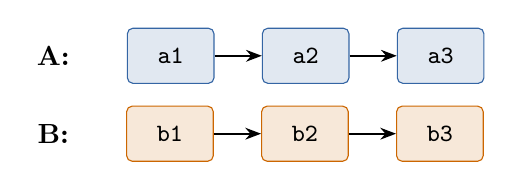
\begin{tikzpicture}[node distance=0.6cm]
  \node (A) {\textbf{A:}};
  \node[la, right=of A] (a1) {a1};
  \node[la, right=of a1] (a2) {a2};
  \node[la, right=of a2] (a3) {a3};
  \draw[arr] (a1) -- (a2); \draw[arr] (a2) -- (a3);

  \node[below=0.5cm of A] (B) {\textbf{B:}};
  \node[lb, right=of B] (b1) {b1};
  \node[lb, right=of b1] (b2) {b2};
  \node[lb, right=of b2] (b3) {b3};
  \draw[arr] (b1) -- (b2); \draw[arr] (b2) -- (b3);
\end{tikzpicture}
\end{center}

\noindent Goal:

\begin{center}
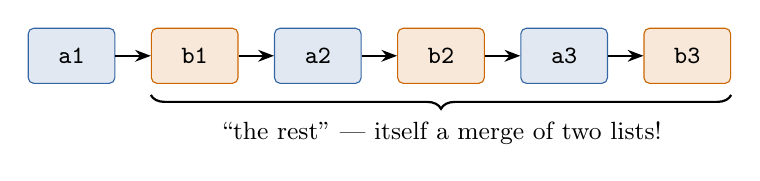
\begin{tikzpicture}[node distance=0.45cm]
  \node[la] (m1) {a1};
  \node[lb, right=of m1] (m2) {b1};
  \node[la, right=of m2] (m3) {a2};
  \node[lb, right=of m3] (m4) {b2};
  \node[la, right=of m4] (m5) {a3};
  \node[lb, right=of m5] (m6) {b3};
  \foreach \i/\j in {m1/m2, m2/m3, m3/m4, m4/m5, m5/m6} \draw[arr] (\i) -- (\j);
  \draw[decorate, decoration={brace, amplitude=5pt, mirror}, thick]
    ([yshift=-4pt]m2.south west) -- ([yshift=-4pt]m6.south east)
    node[midway, below=6pt, font=\small] {``the rest'' --- itself a merge of two lists!};
\end{tikzpicture}
\end{center}

\noindent The result starts with \texttt{a1}, and everything after \texttt{a1} is
\texttt{b1 $\to$ a2 $\to$ b2 $\to$ a3 $\to$ b3}.

\begin{question}
That leftover part is a merge of two lists. \textbf{Which} two lists, and in
\textbf{which order}? (Hint: whose node comes first in the leftover part?)
\end{question}

\section*{Step 2: Base cases \textcolor{green!50!black}{(you already have these)}}

\begin{itemize}[nosep]
  \item If A is empty, the answer is just B.
  \item If B is empty, the answer is just A.
\end{itemize}
These stop the recursion.

\section*{Step 3: The ``leap of faith''}

Recursion works when you \textbf{trust that the function already works on a smaller
input}. Assume \texttt{merge\_orders(X, Y)} correctly merges any two
\emph{shorter} lists. Then ask:

\begin{enumerate}[nosep]
  \item What is the smaller problem? (From Step~1: something built from what comes
        \emph{after} \texttt{a1}, plus list B.)
  \item What order do the arguments go in, so that a \texttt{b} node comes next?
  \item Is at least one argument \textbf{shorter} than before? If not, you will
        recurse forever --- exactly the bug in your current line 28.
\end{enumerate}

\section*{Step 4: Connect the pieces}

Once the recursive call hands back ``the rest of the merged sandwich'':

\begin{question}
\begin{itemize}[nosep, leftmargin=*]
  \item Which node's \texttt{.next} should point to that result?
  \item What do you return as the head of the whole thing?
\end{itemize}
\end{question}

\begin{warn}
If you overwrite a pointer before you have used what it pointed to, you lose the
rest of that list. Think about the \textbf{order} of your steps. Do you need to
save anything in a variable first?
\end{warn}

\section*{Step 5: Trace it by hand}

Before running, trace these on paper. For each call, write down the arguments and
what gets returned.

\begin{center}
\begin{tabular}{lll}
\toprule
\textbf{A} & \textbf{B} & \textbf{Expected} \\
\midrule
\texttt{x}              & \texttt{y}              & \texttt{x $\to$ y} \\
\texttt{x $\to$ z}      & \texttt{y}              & \texttt{x $\to$ y $\to$ z} \\
\texttt{x}              & \texttt{y $\to$ w}      & \texttt{x $\to$ y $\to$ w} \\
\bottomrule
\end{tabular}
\end{center}

\noindent If your traces match, run the real tests.

\section*{Step 6: Fix the test code}

Your merge \textbf{changes the original nodes}. After the first test runs,
\texttt{sandwich\_a} is no longer \texttt{Bacon $\to$ Lettuce $\to$ Tomato}, so the
second test will not print the expected output.

\begin{question}
How can you make sure each test starts with fresh lists?
\end{question}

\section*{Step 7: Complexity}

Let $n$ be the length of A and $m$ be the length of B.

\begin{itemize}
  \item \textbf{Time:} How much work happens in a single call, not counting the
        recursive call? How many calls happen in total?
  \item \textbf{Space:} You create no new nodes, but recursion uses the
        \textbf{call stack}. How many calls can be waiting on the stack at the same
        time?
\end{itemize}

\noindent Write both answers in terms of $n$ and $m$, with a one-sentence reason
for each.

\end{document}
